\section{An\'alisis 3: Universidad de Hamburgo (Alemania)}
Vamos a realizar un an\'alisis de nuestro traceroute sobre la Universidad de Hamburgo.

El host de dicha universidad es http://www.uni-hamburg.de/ (IP: 134.100.56.130 ).\\	


\subsubsection{Par\'ametros de entrada}
\begin{itemize}
\item Host: www.uni-hamburg.de
\item Tiempo Limite: 2
\item Cant. Iteraciones en cada nodo: 15
\item Recorrido m\'aximo de nodos: 25 (TTL m\'aximo)
\item alpha: 0.05
\end{itemize}

\subsubsection{Resultados obtenidos}

Captura general de los resultados obtenidos: 
\\
\\
\newpage
\begin{figure}[h]
	\begin{center}
    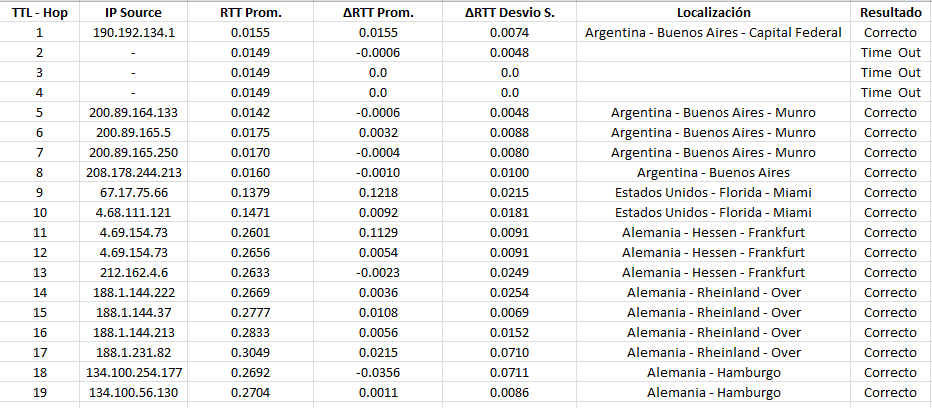
\includegraphics[width=1\textwidth]{img_analisis3/captura.png} 
	\end{center} 
\end{figure}

\subsubsection{An\'alisis de los resultados}
Mediante gr\'aficos haremos un an\'alisis de los resultados obtenidos. \newline


\begin{figure}[h]
	\begin{center}
    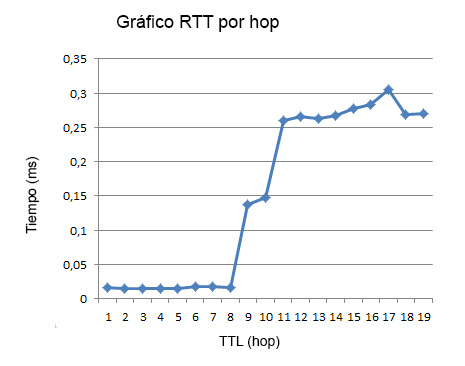
\includegraphics[width=0.7\textwidth]{img_analisis3/grafico-rtt-promedio.jpg} 
    \caption{Figura 1: $RTT$ promedio - Universidad de Hamburgo}	
	\end{center} 
\end{figure}
\newpage
\\
\\
\\


\begin{figure}[h]
	\begin{center}
    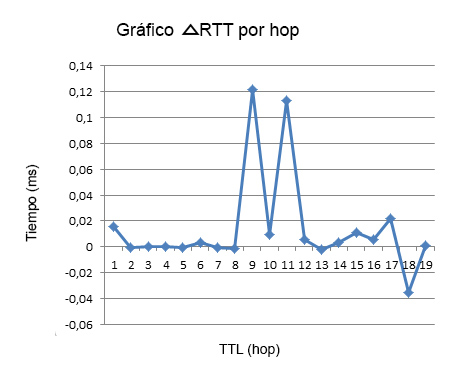
\includegraphics[width=0.7\textwidth]{img_analisis3/grafico-delta-rtt-promedio.jpg} 
    \caption{Figura 1: $\Delta RTT$ promedio - Universidad de Hamburgo}	
	\end{center} 
\end{figure}
%\newline

De la muestra obtuvimos que los $\Delta RTT$ sigen una distribuci\'on Normal y que los enlaces submarinos, según los outliers obtenidos mediante el test de Grubbs, se corresponden con el salto 9 y el 11.
\\
Al observar los gráficos podemos notar que los resultados obtenidos mediante el test de Grubbs son correctos, ya que del salto 8 al 9 el paquete enviado viaja, según la geolocalización de las IP, desde Buenos Aires a Miami y su RTT promedio aumenta significativamente, y del salto 10 al 11 el paquete viaja de Miami a Frankfurt donde también hay un cambio abruto de su RTT promedio.
\\
\\
Finalmente presentamos un mapa global donde vamos a trazar los puntos importantes de la ruta que realizan los paquetes. 

\begin{figure}[h]
	\begin{center}
    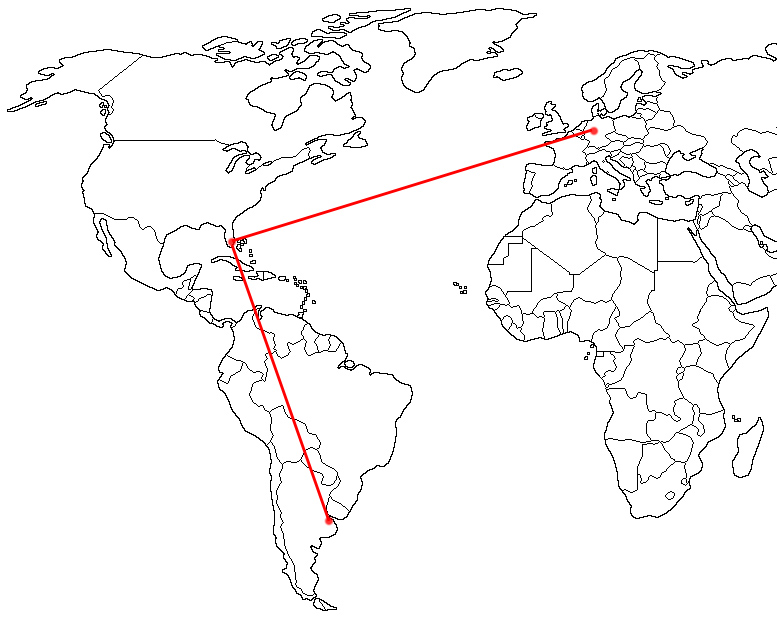
\includegraphics[width=0.7\textwidth]{img_analisis3/mapa.jpg} 
    \caption{Figura 1: Ruta del paquete - Universidad de Hamburgo}	
	\end{center} 
\end{figure}

